\newpage
\section{Suggested solution: Spectral Analysis}

\begin{enumerate}
\item Read the audio file as follows:
\begin{lstlisting}[language=Python]
import scipy.io.wavfile
audio = scipy.io.wavfile.read("b.wav")
sample_rate=audio[0]
# read only one channel of the stereo signal
signal=audio[1][:,0]
\end{lstlisting}

\begin{enumerate}[a)]
\item Using the code given, one can simply print the sample rate. The sample rate is $f_s=44100$ Hz, so the highest and lowest frequencies that can be represented are $f_{s}/2=\pm$22050 Hz.

\item The following code will import the audio file and plot the signal with seconds on the $x$-axis. 
\lstinputlisting[language=Python, caption=Code to plot audio signal,label=code16_4]{ch16/code/ex16_1b.py}

The output of Listing \ref{code16_4} is shown in Figure \ref{audio_plot}.
\begin{marginfigure}
    \centering
    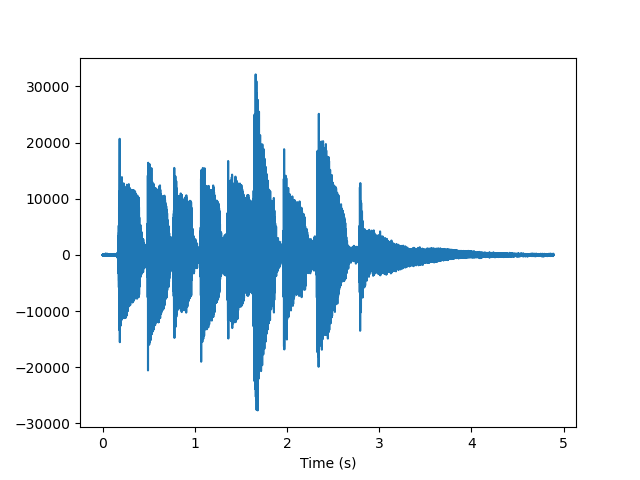
\includegraphics[width=7.5cm,height=7.0cm]{ch16/figures/audio.png}
    \caption{Audio signal}
    \label{audio_plot}
\end{marginfigure}
The length in seconds can be computed as $\text{time in seconds}=(\text{number of samples})(\text{sample spacing})$ which in this case is $t=215678/44100\approx 4.89$, so around a 5 seconds long signal. From Figure \ref{audio_plot} we see that the signal is around 5 seconds long. 

\item The following code shown in Listing \ref{code16_5} will compute and print the spectogram for the audio signal. 

\lstinputlisting[language=Python, caption=Spectogram code, label=code16_5]{ch16/code/ex16_1c.py}

\item The output of Listing \ref{code16_5} is shown in Figure \ref{fur_elise_spectogram}.
\begin{figure}[h!]
    \centering
    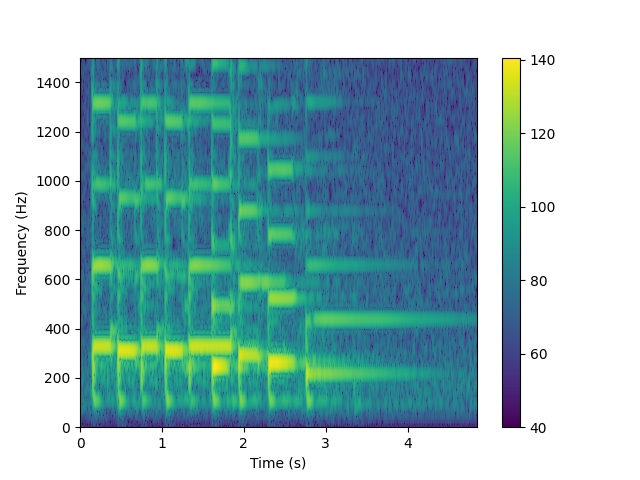
\includegraphics[scale=1.0]{ch16/figures/fur_elise_spectogram.png}
    \caption{Für Elise spectogram}
    \label{fur_elise_spectogram}
\end{figure}

\item Instruments don't produce pure frequency tones, so there will be harmonics, which can be seen in Figure \ref{fur_elise_spectogram}. Different instruments emphasize different harmonics,
giving each instrument its respective sound among other factors. 

\item Comparing the spectogram with the frequency table, one can read that the musical phrase is E D\# E D\# E B D C A. 
You can compare this with sheet music for the piece, which is the correct phrase. 

\end{enumerate}
\end{enumerate}